\section{実験結果}
LoRaWAN (DR2)でのイベントごとの消費電力実測結果を下記\ref{fig:result_power_consumtion}\ref{fig:LoRaWAN_PowerConsumption}に示す.また,LoRaWAN (DR2)でのその他値を下記表\ref{fig:LoRaWAN_Parameter}に示す.パケット到達率は,LoRaWANの送信回数に対してMQTTブローカーで受信したデータ数をもとに算出した.RSSiは,LoRaWANのGWノードが収集しMQTTブローカーに送信するため,その値を参考とした.SNRも同様である.

\begin{figure}[]
    \begin{center}
    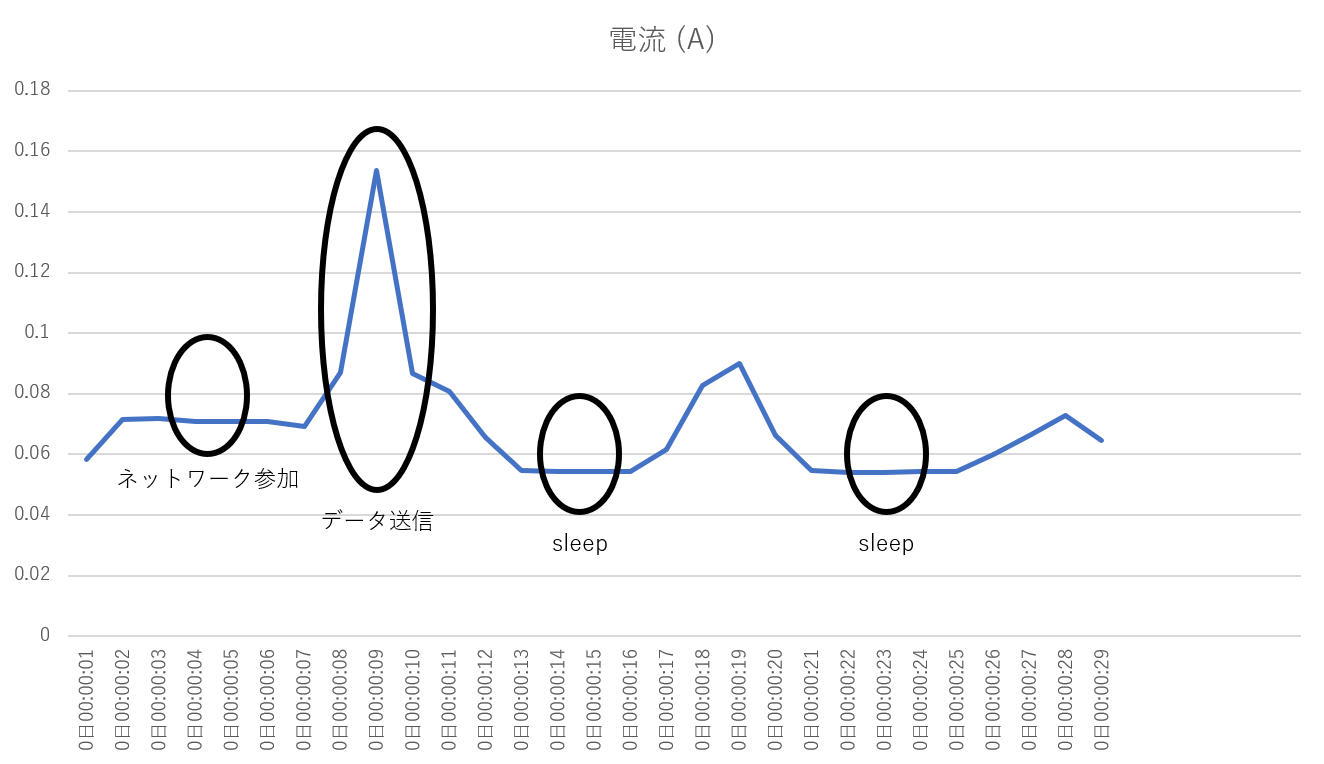
\includegraphics[width=15cm]{figures/LoRaWAN_消費電力実験.png}
    \caption{消費電力測定における各イベント(縦軸:消費電流,横軸:時間(s))}
    \label{fig:result_power_consumtion}
    \end{center}
\end{figure}

\begin{table}[]
    \caption{イベントごとの消費電力}\label{fig:LoRaWAN_PowerConsumption}
    \centering
    \begin{tabular}{|c|l|l|l|}
    \hline
    \textbf{イベント}     & \multicolumn{1}{c|}{\textbf{時間 (second)}} & \multicolumn{1}{c|}{\textbf{電流 (mA)}} & \multicolumn{1}{c|}{\textbf{消費電力 (mW)}} \\ \hline
    起動→ネットワーク参加       & 7                                         & 20                                    & 120                                     \\ \hline
    起動→ネットワーク参加→データ送信 & 11                                        & 21                                    & 105                                     \\ \hline
    スリープ              & なし                                        & 3                                     & 15                                      \\ \hline
    データ送信             & 4                                         & 29                                    & 145                                     \\ \hline
    \end{tabular}
\end{table}

\begin{table}[]
    \caption{その他パラメータ}\label{fig:LoRaWAN_Parameter}
    \centering
    \begin{tabular}{|c|c|}
    \hline
    \textbf{パラメータ} & \textbf{値} \\ \hline
    パケット到達率        & 90\%       \\ \hline
    RSSi           & -102       \\ \hline
    SNR            & -10        \\ \hline
    \end{tabular}
\end{table}